\chapter{Аналитическая часть}

В данном разделе формально описывается процесс продажи вина. Проводится анализ существующих решений. Изучаются и сравниваются существующие модели баз данных и системы управления базами данных. В результате анализа определяются модель базы данных и система управления базами данных, оптимальные для решения поставленной задачи.

\section{Формализация задачи}

Процесс продажи вина состоит из трех основных этапов.

\begin{enumerate}
	\item Поставщик продает вино определенного сорта, цвета, объема и других параметров ритейлеру по закупочной цене $P_{s}$;
	\item Ритейлер выставляет на продажу полученный товар по цене $S$. Цена $S$ называется ценой реализации товара и формируется путем сложения закупочной цены $P_{s}$ и наценки $N$ \cite{pricing}:
\begin{equation}
    S = P_{s} + N;
\end{equation}
Наценка состоит из издержек (оплата услуг по хранению, операций по приведению товара в удобный для продажи вид) и чистого дохода, в который включаются прибыль и налоги \cite{pricing}. 
	\item Покупатель приобретает вино по цене реализации товара $S$, установленной ритейлером. Поставщик получает часть полученной суммы, равную $P_{s}$. Оставшаяся часть уходит на оплату издержек продажи (налоги, оплата труда, другие материальные расходы) $C$. Таким образом, прибыль ритейлера $P_{r}$ формируется следующим образом:
	
\begin{equation}
    P_{r} = S - P_{s} - C,
\end{equation}
\begin{equation}
    P_{r} = P_{s} + N - P_{s} - C,
\end{equation}
\begin{equation}
    P_{r} = N - C.
\end{equation}
\end{enumerate}

Входными данным для процесса виноторговли является структура продукта, выходными --- структура продажи.

\subsection{Структура продукта виноторговли}

Параметры винного продукта могут расширяться в каждом конкретном случае, но основными параметрами являются:

\begin{enumerate}
	\item сорт;
	\item цвет;
	\item объем;
	\item содержание алкоголя;
	\item сахар;
	\item выдержка --- процесс вызревания вина.
\end{enumerate}

Параметры представлены в виде совокупности текстовой информации, как показано в таблице \ref{wine_structure}.

\begin{table}[h]
    \begin{center}
        \begin{threeparttable}
        \captionsetup{justification=raggedright,singlelinecheck=off}
    		\caption{Структура продукта виноторговли}
    		\label{wine_structure}
        \begin{tabular}{|l|l|l|p{30mm}|l|p{25mm}|}
            \hline
            Сорт & Цвет & Объем (л) & Содержание алкоголя (\%)  & Сахар & Выдержка (год) \\ \hline
            Ламбруско & Белый & 0.75 & 8 & Полусладкое & 2 \\ \hline
        \end{tabular}
    \end{threeparttable}
    \end{center}
\end{table}

\subsection{Структура продажи}

Для учета всех составляющих процесса продажи структура должна содержать следующие параметры:

\begin{enumerate}
	\item идентификатор продукта;
	\item идентификатор поставщика;
	\item идентификатор покупателя;
	\item закупочная цена $P_{s}$;
	\item цена реализации $S$;
	\item наценка $N$;
	\item сумма издержек $C$;
	\item прибыль $P_{r}$;
	\item дата продажи.
\end{enumerate}

Параметры представлены в виде совокупности текстовой информации, как показано в таблице \ref{sale_structure}. Параметры №4-№8 указаны в рублях.

\begin{table}[h]
    \begin{center}
        \begin{threeparttable}
        \captionsetup{justification=raggedright,singlelinecheck=off}
    		\caption{Структура продажи}
    		\label{sale_structure}
    		\footnotesize
        \begin{tabular}{|p{25mm}|p{25mm}|p{25mm}|l|l|l|l|l|p{15mm}|}
            \hline
            Идентификатор продукта & Идентификатор поставщика & Идентификатор покупателя & $P_{s}$ & $S$ & $N$ & $C$ & $P_{r}$ & Дата продажи\\ \hline
            3 & 1 & 100 & 500 & 650 & 150 & 50 & 100 & 09.09.2022 \\ \hline
        \end{tabular}
    \end{threeparttable}
    \end{center}
\end{table}

\section{Формализация ролей}

Участниками виноторговли, которые будут использовать информационную систему, являются поставщик вин и покупатель. Для управления их запросами в информационной системе необходим администратор.

Для поставщика определены следующие действия:

\begin{itemize}
	\item регистрация в системе;
	\item вход в аккаунт;
	\item выход из аккаунта;
	\item получение данных:
		\begin{itemize}
			\item о вине;
			\item о продажах;
		\end{itemize}		 
	\item создание запроса:
		\begin{itemize}
			\item на добавление нового товара;
			\item на удаление товара;
			\item на редактирование товара.
		\end{itemize}
\end{itemize}

В возможности покупателя входит:

\begin{itemize}
	\item регистрация в системе;
	\item вход в аккаунт;
	\item выход из аккаунта;
	\item получение данных:
		\begin{itemize}
			\item о вине;
			\item о поставщике;
			\item о рейтинге вин;
			\item о покупках;
		\end{itemize}
	\item создание запроса на получение бонусной карты.
\end{itemize}

Администратор обладает правами на следующие действия:

\begin{itemize}
	\item вход в аккаунт;
	\item выход из аккаунта;
	\item получение данных:
		\begin{itemize}
			\item о вине;
			\item о продажах;
		\end{itemize}
	\item одобрение или отклонение:
		\begin{itemize}
			\item выдачи бонусной карты пользователю;
			\item добавления товара поставщика;
			\item удаления товара поставщика;
			\item редактирования товара поставщика.
		\end{itemize}
\end{itemize}

\section{Формализация данных}

С учетом выделенных структур данных и типов пользователей разрабатываемая база данных должна содержать информацию о следующих данных:

\begin{itemize}
	\item вина;
	\item поставщики;
	\item покупатели;
	\item администраторы;
	\item продажи;
	\item бонусные карты покупателей;
	\item покупки покупателей.	
\end{itemize}

\section{Анализ существующих решений}

Компании-ритейлеры в сфере виноторговли предоставляют интернет-магазины алкогольных напитков.

\subsection{Российский рынок}

Интернет-магазины российских специализированных сетей "ВинЛаб" \cite{winelab}, "Красное\&Белое" \cite{kb} и других предоставляют возможности 
регистрации в системе покупателей, просмотра информации о спиртных напитках, покупках, составления рейтинга и получения бонусной карты. Кроме того, в каталогах представлена информация не только о винах, но и о других алкогольных напитках.

\subsection{Зарубежный рынок}

Зарубежные компании-ритейлеры "Primal Wine" \cite{primal_wine} и "Wine.com" \cite{wine_com} реализуют продажу только вина. В системе можно зарегистрировать аккаунт покупателя, получать информацию о винах и составлять рейтинги по различным параметрам. Покупатель может стать участником винного клуба, получив персонализированную подписку на вино. 

\subsection{Вывод}

Как на российском, так и на зарубежном рынке существуют сервисы, автоматизирующие продажу вин, расчитанные только на покупателей, но не предоставляющие функциональность для поставщиков. Таким образом, полноценных существующих решений не найдено.

\section{Анализ БД}

\section{Анализ СУБД}

\section{Вывод}

\chapter{Конструкторская часть}

\begin{figure}[H]
	\begin{center}
		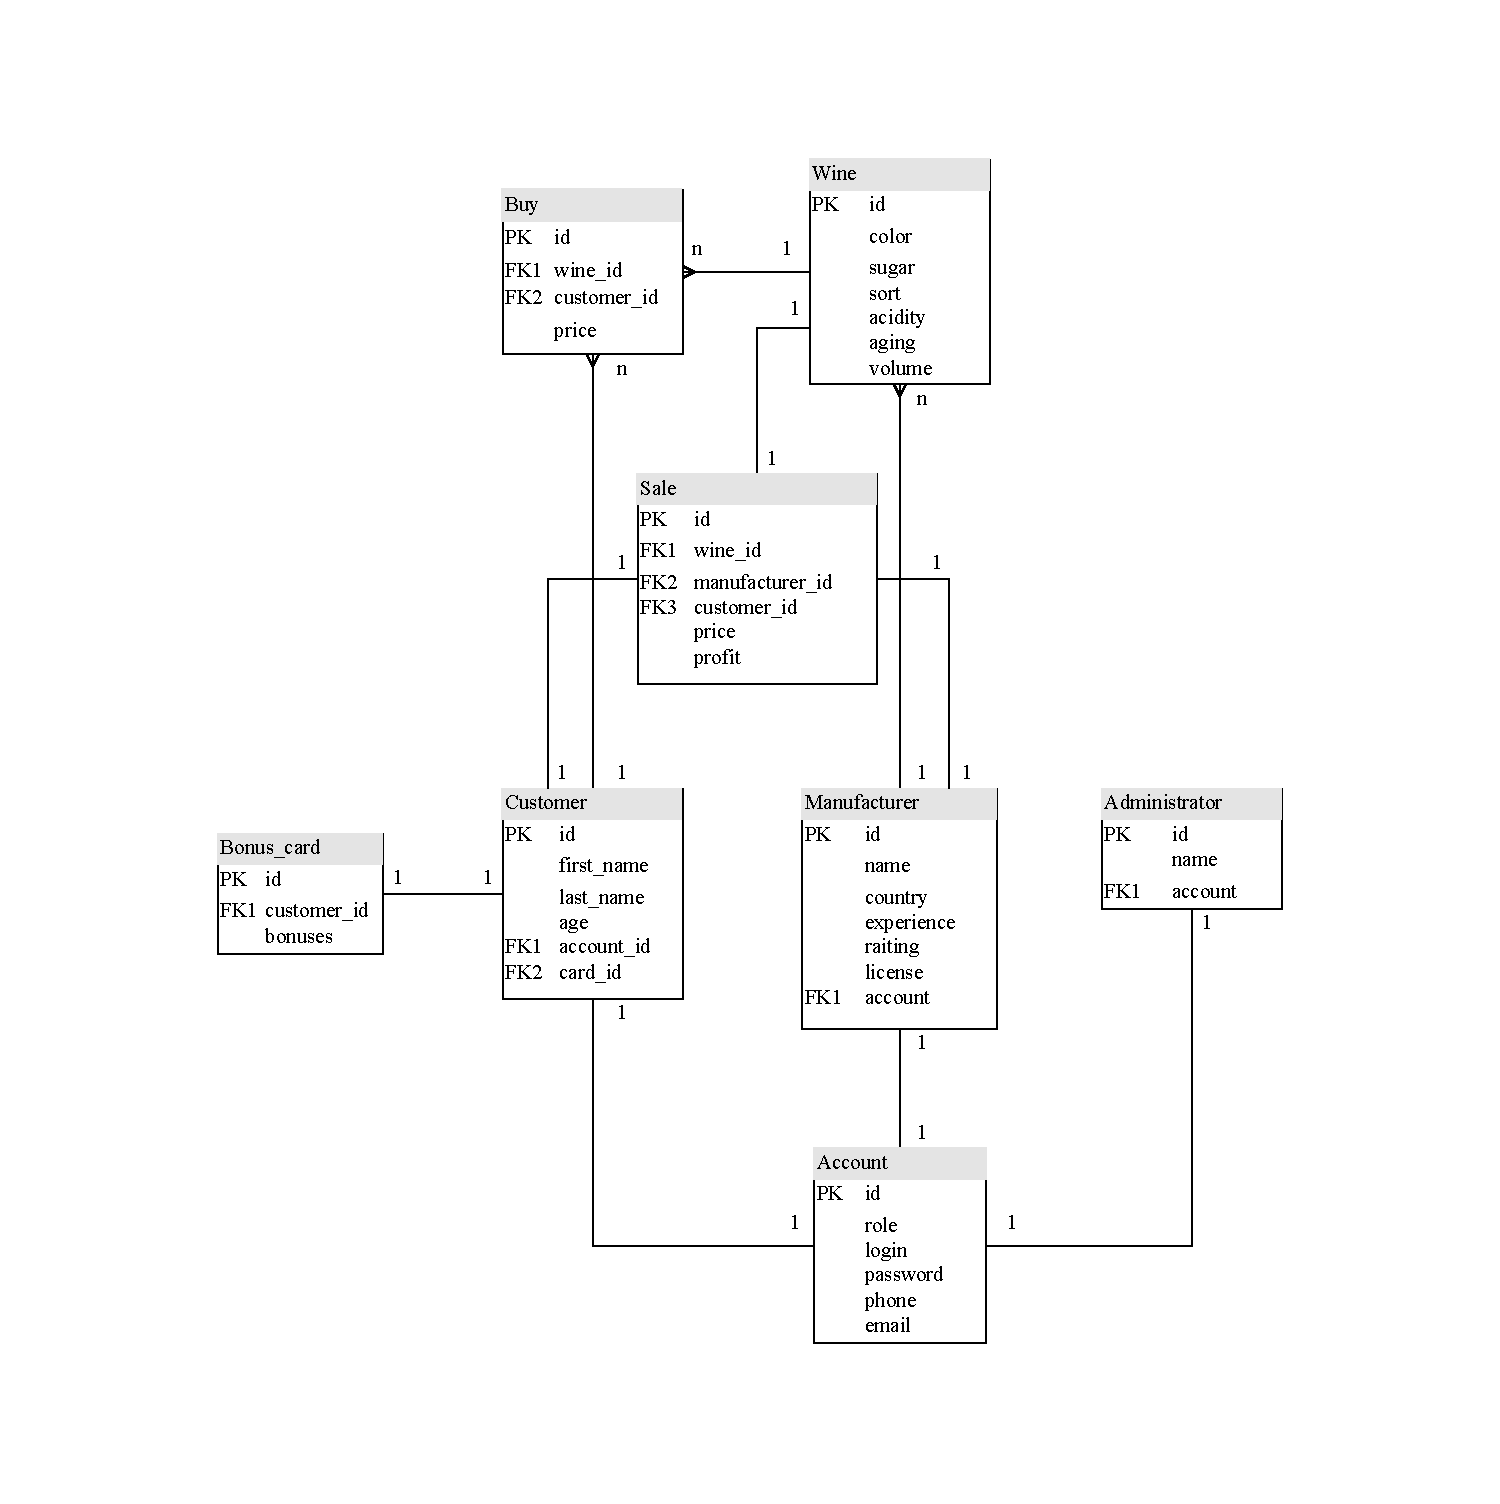
\includegraphics[scale=0.75]{img/ER-diagram.pdf}
	\end{center}
	\captionsetup{justification=centering}
	\caption{ER-диаграмма сущностей}
	\label{img:er}
\end{figure}

\section{Use-case диаграммы}

\begin{figure}[H]
	\begin{center}
		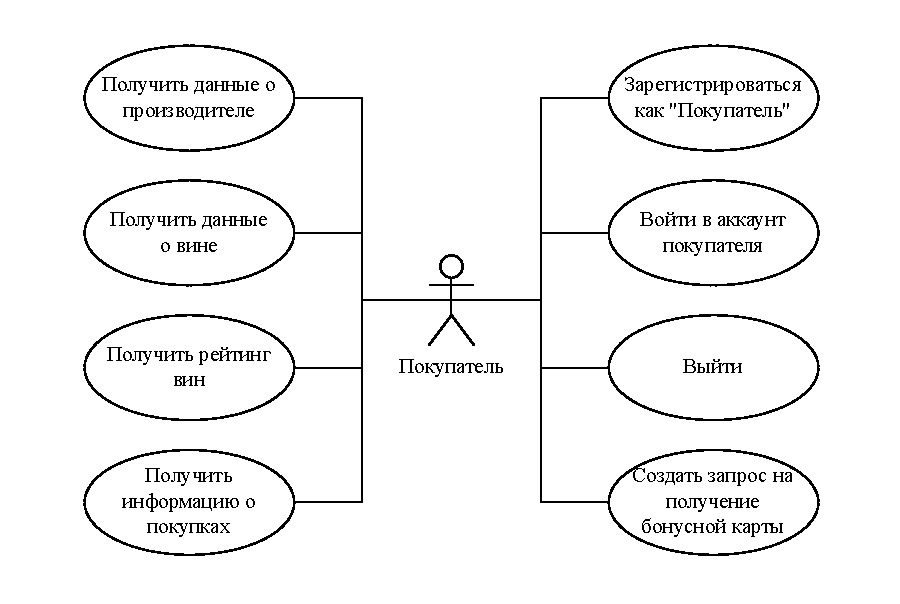
\includegraphics[scale=0.8]{img/customer.pdf}
	\end{center}
	\captionsetup{justification=centering}
	\caption{Use-case - покупатель}
	\label{img:customer}
\end{figure}

\begin{figure}[H]
	\begin{center}
		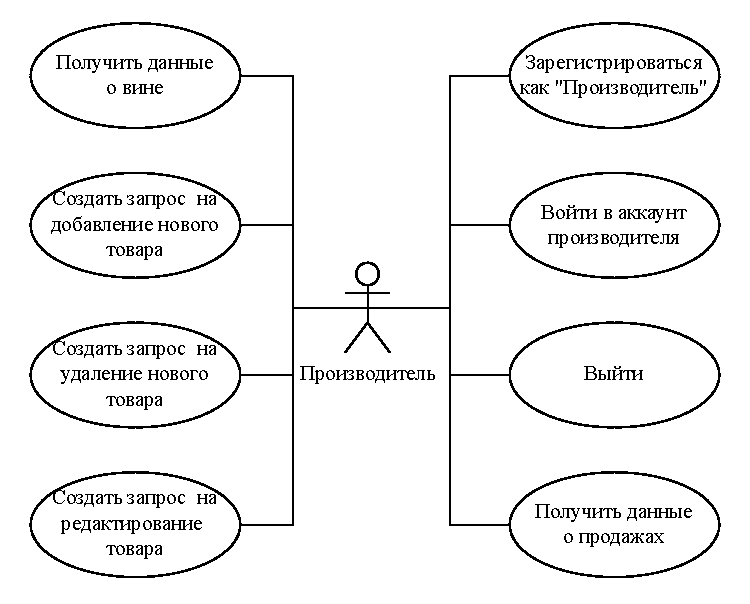
\includegraphics[scale=0.8]{img/manufacturer.pdf}
	\end{center}
	\captionsetup{justification=centering}
	\caption{Use-case - производитель}
	\label{img:manufacturer}
\end{figure}

\begin{figure}[H]
	\begin{center}
		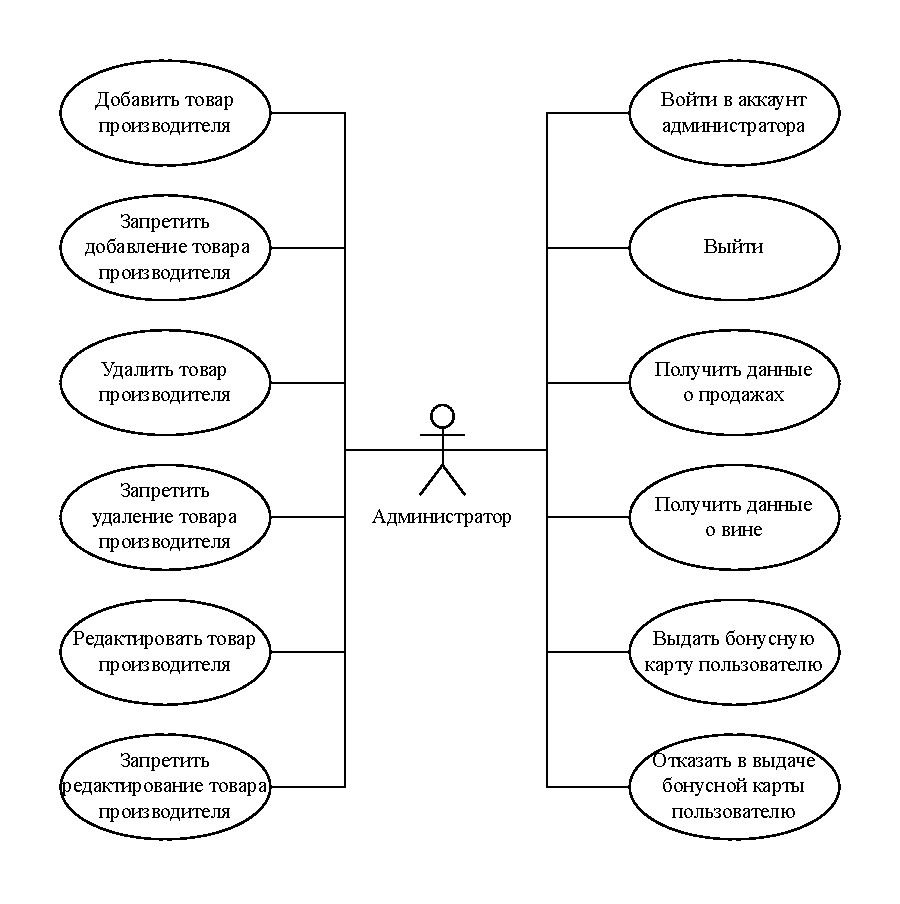
\includegraphics[scale=0.8]{img/administrator.pdf}
	\end{center}
	\captionsetup{justification=centering}
	\caption{Use-case - администратор}
	\label{img:administrator}
\end{figure}